\chapter[The identity issue]{Who's who? The identity issue}
\label{ch:identity}
\textbf{Identity} is a fundamental component of security; we cannot presume to realize a secure system if we do not take into account this issue, because we must know \textit{who is who}. The very basic idea of security is to allow authorized people to do their stuff, and forbid everybody else from doing the same things - and this requires \textbf{identification}.

%----------------------

\subsubsection*{Recap}
We saw in chapter \ref{ch:intro_crypto} many different ways of securing a communication between two (or more) people or devices:

\begin{itemize}
    \item \textbf{HASH}: useful only when using different channels;
    \item \textbf{HMAC}: safer than HASH, but we need a secret key;
    \item \textbf{symmetric cryptography}: good, but we need a secret key and, more importantly, cannot tell who is who (we cannot trust \textit{both} ends);
    \item \textbf{asymmetric cryptography}: good, but we still need to identify the involved parties; also, it is slower than symmetric cryptography.
\end{itemize}

Note that having a secret key does not mean that we can identify people or devices; the key does not tell anything about who we are: anybody who has it can pretend to be us.

%----------------------------------------------------------------------------------------

\section{The identity issue}
The \textbf{identity issue} comes down to the one major problem of ensuring that the identity of a person or device is correct, and not counterfeited. Basically, we want and need to know that if someone is claiming to be someone, then it is true.

The trick to do this to tie \textbf{something} to someone's identity, like an ID card containing a photo of the person it belongs to, which can be later used to identify that person.

%-------------------------------------------

\subsection*{The identity issue in humans}
This is a very old problem, related to administrative issues. Who ensures us that our friend is the person he or she claims to be? Nobody, really. We trust that they are who they say they are because they presented themselves to us that way, and everybody else calls them by the name they introduced themselves with.

As humans, we are always identified by someone else: whoever identifies us from our documents matches our appearance to the photo on our ID card, trusting that the document contains rightful information (assuming that it has been printed the right way, that it has all necessary stamps and that somebody at the municipal office verified that everything was right). Ultimately, it always is a matter of \textbf{trust}.

Identity verification during a system login is different depending on whether we are a human or a computer; humans normally have more possibilities, among which the infamous \textbf{three} (sometimes two) \textbf{factor authentication}:

\begin{itemize}
    \item something we \textbf{know} (a password);
    \item something we \textbf{have} (a smart card, a phone, etc.);
    \item something we \textbf{are} (a fingerprint or other biometric method).
\end{itemize}

%-------------------------------------------

\subsection*{The identity issue in computers}
Regarding computers, the best thing to identify them is to use \textit{something they know} (a secret key), because it is difficult to ask them about \textit{something they have} (they would need some physically attached peripheral in order to do this). It is important to note that keys are not a real proof of identity, but rather a way to discriminate between different devices; we rely on keys because generating two identical keys is extremely improbable but still, the fact that we can distinguish between two or more devices does not mean that they are really who they say they are.

In computers we have to rely on some assumptions. For example, we suppose that from an administrative point of view somebody ensures that a private key is private, and thus that the admin did not install someone else's identity, and that our own identity has only been installed on our computer. But how can we be sure that a certain private key belongs to a certain owner? A way to do this is using \textbf{fingerprints}, a meta-information that goes beyond the key and tells us something about the entity itself (device, program, etc.).

In telecommunications, \textbf{fingerprints} are part of a cryptographic key; they are not meant to decrypt anything, but instead work like a hash. The only difference between a fingerprint and a hash is that while the hash gets a message in input and spits out another, coded one, a fingerprint is just a part of somebody's secret key. Fingerprints are always contained in public keys, so that their owner can give them out to as many users as possible, thus allowing people and devices to identify the owner itself and giving a hard time to attackers to mess up with them (they could modify some, but not \textit{all} existing fingerprints). Of course, this method is only reliable as long as the recipient actively searches for the fingerprint, otherwise it could receive a tampered one but would not notice it.

In practice: we hash the key and some more data (like the key length, the cypher method, etc.), then use it as a fingerprint. This method is better than using directly the key, because it is much shorter: while a private key is usually 256 bytes long, a SHA1 fingerprint is only 20 bytes long.

%----------------------------------------------------------------------------------------

\section{Web of trust}
Another way of ensuring someone's identity is to trust who is already trusted by others, like we do everyday in real life; basically searching for a consensus. For example, suppose we generate our own key; since we know and trust our colleagues in the next room, we have them generate their keys, too, and then sign each other's key (by generating an HMAC). A \textbf{web of trust} is thus a concept used to establish the authenticity of the binding between a public key and its owner, and in its most basic form it works as shown in figure \ref{fig:wot}.

\begin{figure}[h]
    \centering
    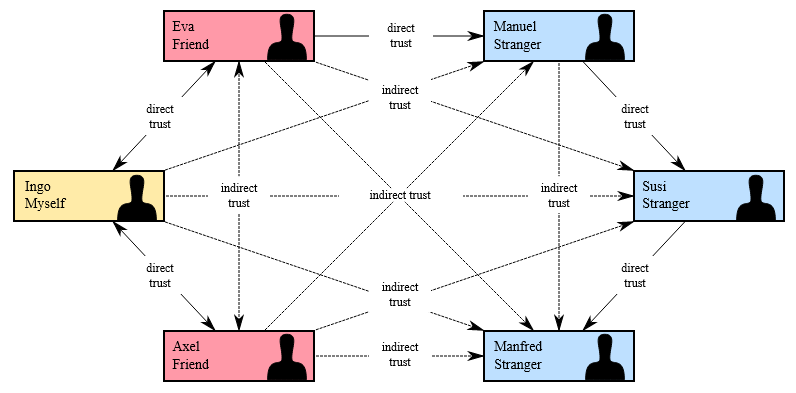
\includegraphics[scale=0.8]{img/wot.png}
    \decoRule
    \caption{Schematic diagram of a web of trust.}
    \label{fig:wot}
\end{figure}

The problem with web of trusts is that a group large enough can subvert it, meaning that it can inject in another system stuff that will be considered true by other people. Basically, we are trusting that other people did not sign a forged document (it is a shared trust), but when enough people believe that even for a forged document, because for some reason they have been fooled, then others who trust them will be fooled, too, because they trust the wrong people. In these cases there is nobody to blame if we receive wrong information: it is not a technical, but an administrative issue.

%----------------------------------------------------------------------------------------

\section{Certificates}
A \textbf{certificate} is something that is not signed by peers, but by a \textbf{Certification Authority} (\textbf{CA}). Instead of having private and public keys, we have some information (written in the X.509 format\footnote{\label{foot:x500}X.500 is a series of networking standards covering electronic directory services. Its primary concept is that there is a single hierarchical organization of entries (a Directory Information Tree, DIT) which are distributed across one or more servers (Directory System Agents, DSA). An entry consists of a set of attributes, each of which with one or more values.}) signed by a higher entity trusted by everybody (which in this case \textit{can} be blamed), which has been \textbf{delegated} to verify a document's authenticity. For this reason certificates have a single signature (instead of multiple ones, like in a web of trust) - not because it is stronger, but because the higher entity is trustworthier than our peers.

Let us see how a certificate is made; even though its structure is not important, it can help us better understand how it works.

\begin{figure}[h]
    \centering
    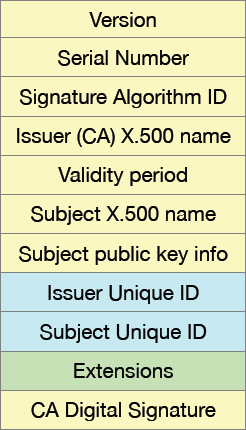
\includegraphics[scale=0.5]{img/ca_structure.png}
    \decoRule
    \caption{Structure of a certificate.}
    \label{fig:ca_structure}
\end{figure}

Figure \ref{fig:ca_structure} depicts a typical certificate; the yellow parts are common to all versions, the blue ones are only available to the second version of the standard, while extensions are only supported by the third version. There are three versions of certificates, all of them backwards compatible (older versions just skip the parts that they do not understand). Let us analyze in detail each component of a certificate:

\begin{itemize}
    \item \textbf{Version}: the version used for the certificate (first, second or third);
    \item \textbf{Serial number}: number of the certificate; it is \textit{not} globally unique, but only among the certificates issued by that authority;
    \item \textbf{Signature algorithm ID};
    \item \textbf{Issuer X.500 name}: this is the name of the CA (e.g. Poste Italiane, VeriSign, etc.), in X.500 format\footref{foot:x500};
    \item \textbf{Validity period}: certificates have an expiration date, after which they are not valid anymore;
    \item \textbf{Subject X.500 name}: this is the main reason of the certificate's existence: it associates the public subject's key with its name (an example could be the following: the host's subject name is \texttt{www.dinfo.unifi.it}, its public key is \texttt{<public key>}, and the subject's X.500 name is \texttt{<public key info>});
    \item \textbf{Subject public key info}: information about the subject's public key (algorithm used, key size, key usage and the public key itself);
    \item \textbf{Issuer Unique ID}: needed to avoid ambiguity among issuers;
    \item \textbf{Subject Unique ID}: needed to avoid ambiguity among subjects;
    \item \textbf{Extensions}: extensions to the certificate, that hold additional information;
    \item \textbf{CA Digital Signature}: just like in a web of trust, this signature is hold as being true because the CA has generated a hash of the certificate itself, encrypted it with its private key and put it in this field.
\end{itemize}

The validity period is very important, because it means that after a period of time the certificate cannot be trusted anymore. This is needed because a certificate's public key, given enough time, can be broken by an attacker; invalidating the certificate after some time ensures that attackers have not had enough time to find a private key that matches the public one.

%-------------------------------------------

\subsection{Use of certificates}
Certificates are simple: the user generates an asymmetric key, and then the key and the user’s identity are signed by the CA. So instead of sending out only a public key, we send out a certificate, which along with our public key also contains more information about our identity, allowing for a better identification. Clearly, if we possess the matching private key, then we have a true identity.

How to verify if the certificate is valid? We can recalculate the CA's digital signature and verify if the hash is right. If the certificate has been created with a CA's private key, in order to do this we can use the CA's public key to decrypt it and see if everything matches. But at this point how can we ensure that the public key given to us by the CA is trustable? It looks pretty much like a cat chasing its tail.

The solution to this problem is for us to \textit{already} possess the CA's public key, by having it \textit{preinstalled} in our computer by the operating system.


It is obvious that the OS must be trustable (meaning that it has not been compromised in any way), because if we get the key of a fake CA then we will automatically trust any certificate signed by that CA, making an attacker very happy. For this reason we should always install security updates, which often contain new CA keys that replace older, expired ones.

From a technical point of view, certificates are \textit{not} better than webs of trust, but still, they allow us to have somebody to blame whenever things go wrong.

%-------------------------------------------

\subsection{Revocation}
Certificates might be deleted for many reasons: the CA stopped operations, their site was put down, etc., and thus we have to invalidate a certificate. The problem with doing this is that anybody who still has that certificate can re-broadcast it, and we cannot just say to everybody to stop using it (there would be too many people, and we would not even know who is using it). The certificate must then be revoked through a \textbf{Certification Revocation List} (\textbf{CRL}) hosted by the CA, and check every time if a certificate we are using is on that list.


We should always ask the CA if a certificate is valid; the downsides are that instead of having a communication between A and B, we also involve the CA, which means slower connection, increased traffic to the CA and a loss of privacy (e.g. if we ask the CA if our bank certificate is valid, they would know how many people are using a certain bank, which is valuable information, and might also do something like the DNS or web browsers, which are capable of collecting our web history at domain level).

%-------------------------------------------

\subsection{Compromised CAs}
A compromised certification authority (i.e. the private key of the CA went into the wrong hands) represents a huge problem, because if somebody has this key they can create certificates for anybody and anything (like, really anything). This means that the CA has to ensure that its private keys are kept private, and that it never ever uses them to generate fake certificates (which has already happened many times); if a CA does questionable things, then it faces a public ban on the Internet, and for example web browsers will stop accepting their certificates (or they could be pulled from operating systems).

%-------------------------------------------

\subsection{Use of certificates in browsers}
Certificates are mostly used in browsers, in the \textbf{HTTPS} protocol (Hypertext Transfer Protocol Secure). HTTPS is an extension of the Hypertext Transfer Protocol (HTTP) used for secure communication over a network, and is widely used on the Internet. Basically, the communication protocol is encrypted using Transport Layer Security (TLS) (or, formerly, Secure Sockets Layer, SSL), and thus it is also referred to as \textit{HTTP over TLS} (or \textit{HTTP over SSL}).

In practice, instead of creating a TCP socket to communicate end-to-end, we create a TLS socket, which is located between the application layer (layer 7) and the TCP protocol. TLS is an enormous protocol: it does a lot of things, and among others it creates a secure channel (not mandatorily encrypted).

All versions of TLS use certificates; TLS sockets however, are exactly like a TCP socket (except for the initialization, where we also have to state things like which version we want, if we want to trust just the certificate sent to us or if both parts need certificates, if we need to identify who sent the certificate, etc.). We could have e-mail, IMAP, SMTP, etc. over TLS: certificates are not only used in web browsers.